%!TEX root = ../main.tex

\section{More Graphs}

\begin{definition}
    (Informal) Biconnected components are "maximal" pieces of the
    graph that are biconnected.
\end{definition}

Let's define an equivalence relation $R$ on $E \times E$ where
$(e_1, e_2) \in R$ if and only if there exists a simple cycle that
contains $e_1$ and $e_2$ (Exercise: show it's an equivalence
relation). $R$ partitions the edges into equivalence classes $E_1,
..., E_k$. Note that if $R$ only has one equivalence class then the
graph is biconnected. Let component $G_i$ be the graph containing edges in
$E_i$ together with the vertices in $V_i$ consisting of the endpoints
of $E_i$.

Let's go back to DFS. Assume $G$ is connected and start DFS at node
$s$. When is $s$ an articulation point?

\begin{itemize}
    \item Case 1: $s$ has only one child in the DFS tree. In this case
    $s$ is not an articulation point.
    \item Case 2: $s$ has more than one child. Then $s$ is an
    articulation point because non-tree edges go between ancestors and
    descendants. In other words, any vertex in the subtree
    generated by one child of $s$ must
    go through $s$ to reach any vertex in the subtree of another
    child of $s$.
\end{itemize}

What conditions make any vertex $v$ in the DFS tree of $s$ an
articulation point? Suppose $v$ has children $u_1, u_2, ..., u_k$.
An internal node $v$ is an articulation point if and only if
it has a child $u_i$ such that there is no back edge from the subtree
rooted at $u_i$ to a proper ancestor of $v$. See Figure~\ref{fig:articulation} for a diagram.

\begin{figure}
    \centering
    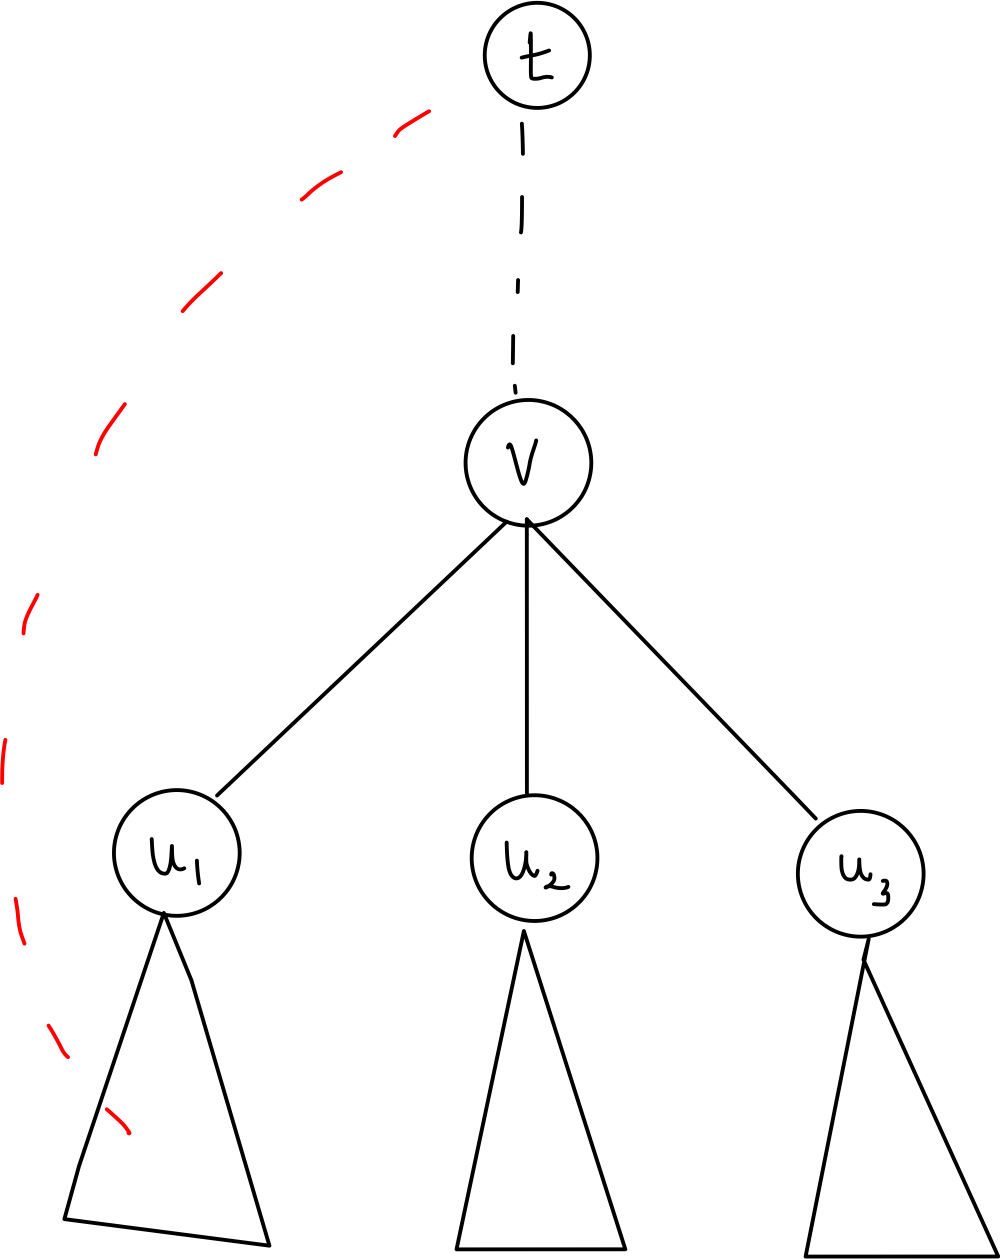
\includegraphics[width=0.3\textwidth]{figures/articulation.jpeg}
    \caption{Condition that makes $v$ an articulation point. In this
    case, it is because the subtree generated by a child of $v$ has a
    back edge to an ancestor of $v$.}
    \label{fig:articulation}
\end{figure}

\subsection{Finding Biconnected Components}

We first must do a DFS starting on a source $s$ and we must do a post
order traversal of the DFS tree as it is produced. As it finds
biconnected components, it outputs them.

Recall that if $u$ is an ancestor of $v$ in the DFS tree, then the
start times $s(u) < s(v)$. Define $\text{low}(x)$ as 
the smallest number (start time) vertex reachable by a back edge from
the subtree rooted at $x$. Suppose for simplicity $v$ has only two
children $u_1, u_2$. Then 

$$
\text{low}(v) = \min(\text{low}(u_1), \; \text{low}(u_2),
\; \underbrace{s(u) : \text{$(v, u)$ is a back edge}}_{\text{we must
consider the back edges of $v$}})
$$

\begin{lemma}
    An internal node $v$ is articulation point if and only if there
    is a child $u_i$ of $v$ such that $\text{low}(u_i) \geq s(v)$.
\end{lemma}

\section{Directed Graphs}

In directed graphs, edges are ordered pairs, so that $(u, v) \in E$
means $u$ is directed to $v$. Naturally, algorithms that we talked
about for undirected graphs might change for directed graphs. Consider
DFS for a directed graph. What type of edges do you encounter? You can
have forward edges, back edges or cross edges. An example of a cross
edge can be seen in Figure~\ref{fig:cross-edge}.

\begin{figure}[hpt]
    \centering
    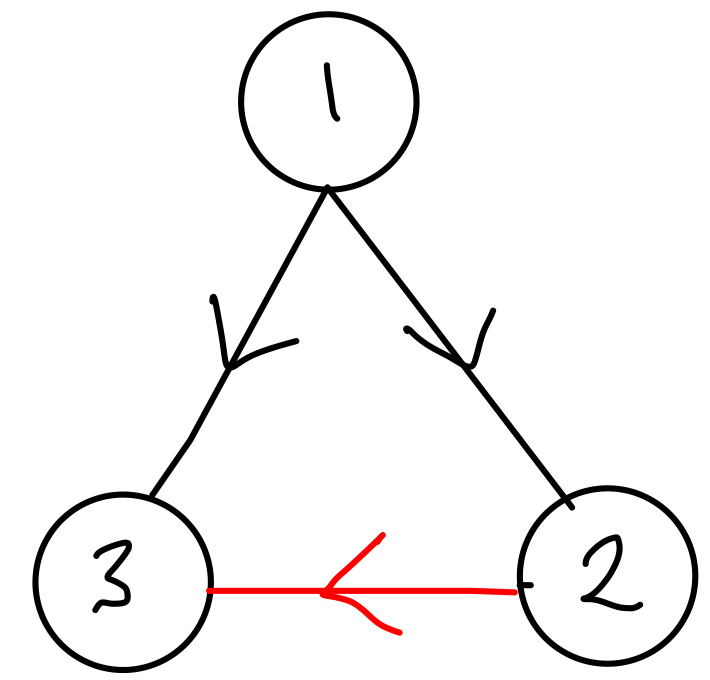
\includegraphics[width=0.2\textwidth]{figures/cross-edge.jpeg}
    \caption{Example of a cross edge in red.}
    \label{fig:cross-edge}
\end{figure}

If $(u, v)$ is a cross edge, then $s(u) > s(v)$.

\subsection{Directed Acylic Graphs (DAGs)}

An example of a DAG is your university course dependency graph, where
some nodes have precedence over others. In general, our goal is to
find an ordering of the vertices such that for each edge $(u, v)$
we have that $u$ precedes $v$ in the ordering. This problem is called
\textbf{topological sorting}.

\begin{lemma}
    Any DAG has a topological ordering.
\end{lemma}

\begin{proof}
    Exercise. Use induction. Or contradiction.
\end{proof}

\begin{definition}
    The in degree of a vertex is the number of incoming edges.
\end{definition}

\begin{theorem}
    If $G$ is a DAG and $(u, v)$ is an edge then for any DFS,
    $f(u) > f(v)$.
\end{theorem}

\begin{proof}

    We show $f(u) > f(v)$.
    \begin{itemize}
    \item Case 1: $s(u) < s(v)$. Then $v$ will become a descendant of
    $u$ (not necessarily a child), so then $f(u) > f(v)$.
    \item Case 2: $s(u) > s(v)$. If we discovered $u$ in the course
    of DFS of $v$, then there must be a path from $v$ to $u$, which
    means $G$ has a cycle, and this is a contradiction. Therefore, 
    $s(v) < f(v) < s(u) < f(u)$
\end{itemize}
In both cases, $f(u) > f(v)$.
\end{proof}

\begin{remark}
    Once you prove this theorem, finding a topological sort of a DAG is
very easy. Find the finish time of all the vertices and output them
in reverse finish time order.
\end{remark}














